\chapter{Introduction}
There is currently strong interest in the development of distributed video
   analysis systems that can be used to analyze large video databases.
Unfortunately, the overwhelming majority of computer systems
   have not been designed and will not efficiently handle
   the basic problem of scalable and distributed video analysis.
   
An example of a large-scale video database is 
   provided by the
   advancing out of school learning in mathematics and engineering (AOLME)
   project.
AOLME contains over a thousand hours of high quality video
   data that need to be analyzed so as to understand how
   middle-student acquire basic programming skills.
Currently, most of this analysis is done manually \cite{LopezLeiva2016}. 

Manual video annotation and transcription
   is extremely tedious and unsustainable for large datasets.    
Because of these inhibitory factors, most of
   these encoded videos are left untouched and unanalyzed, potentially leaving
   thousands of hours of valuable information about the learning process unexplored
   and  underutilized. 
Clearly there is a need for a tool to aid researchers in
   properly analyzing these video datasets efficiently.

\section{\label{section:motivation}Motivation}

Current methods in video analysis systems 
   are extremely application dependent and are inadequate
  computationally and in scalability to sufficiently investigate video datasets at such
a large scale. As such, there is a propensity for a system that is accurate,
scalable and flexible in nature to handle a variety of problems currently faced
with automated video analysis.

Computationally, there is clearly a need for video analysis methods that can be
efficiently implemented in heterogenous compute hardware (such as GPUS and
CPUS), and have said hardware function in a distributed environment. Being able
to leverage heterogenous computer hardware greatly increases the efficiency and
speed of certain, heavily used, video processing algorithms such as 2D
convolutions. Furthermore, having this system exist in a distributed environment
will greatly speed up ephemeral operations and makes it possible to scale up
to address larger scale problems.
Thus this thesis is motivated
   by the challenges associated with analyzing large scale video databases.

\section{\label{section:thesis_statement}Thesis Statement}
The thesis of this research is that it is possible to scale, accurately
  classify and process videos using
  the video interactively and distributively analyzed (VIDA) system.
The basic idea is to effectively distribute the computation among
  compute nodes and collect the results in the master node.
The focus will be to pre-compute the computationally intensive
  feature-extraction
   
  
such as Farneback, Lucas-Kanade optical flow and SVMs powered by a highly scalable
computing architecture, we show that large amounts of video data can be
accurately classified and that our technique is scalable. Figure \ref{fig:typing_writing}
illustrates the types of pre-cropped videos that we are attempting to classify.

\begin{figure}[h]
  \label{fig:typing_writing}
  \centering
  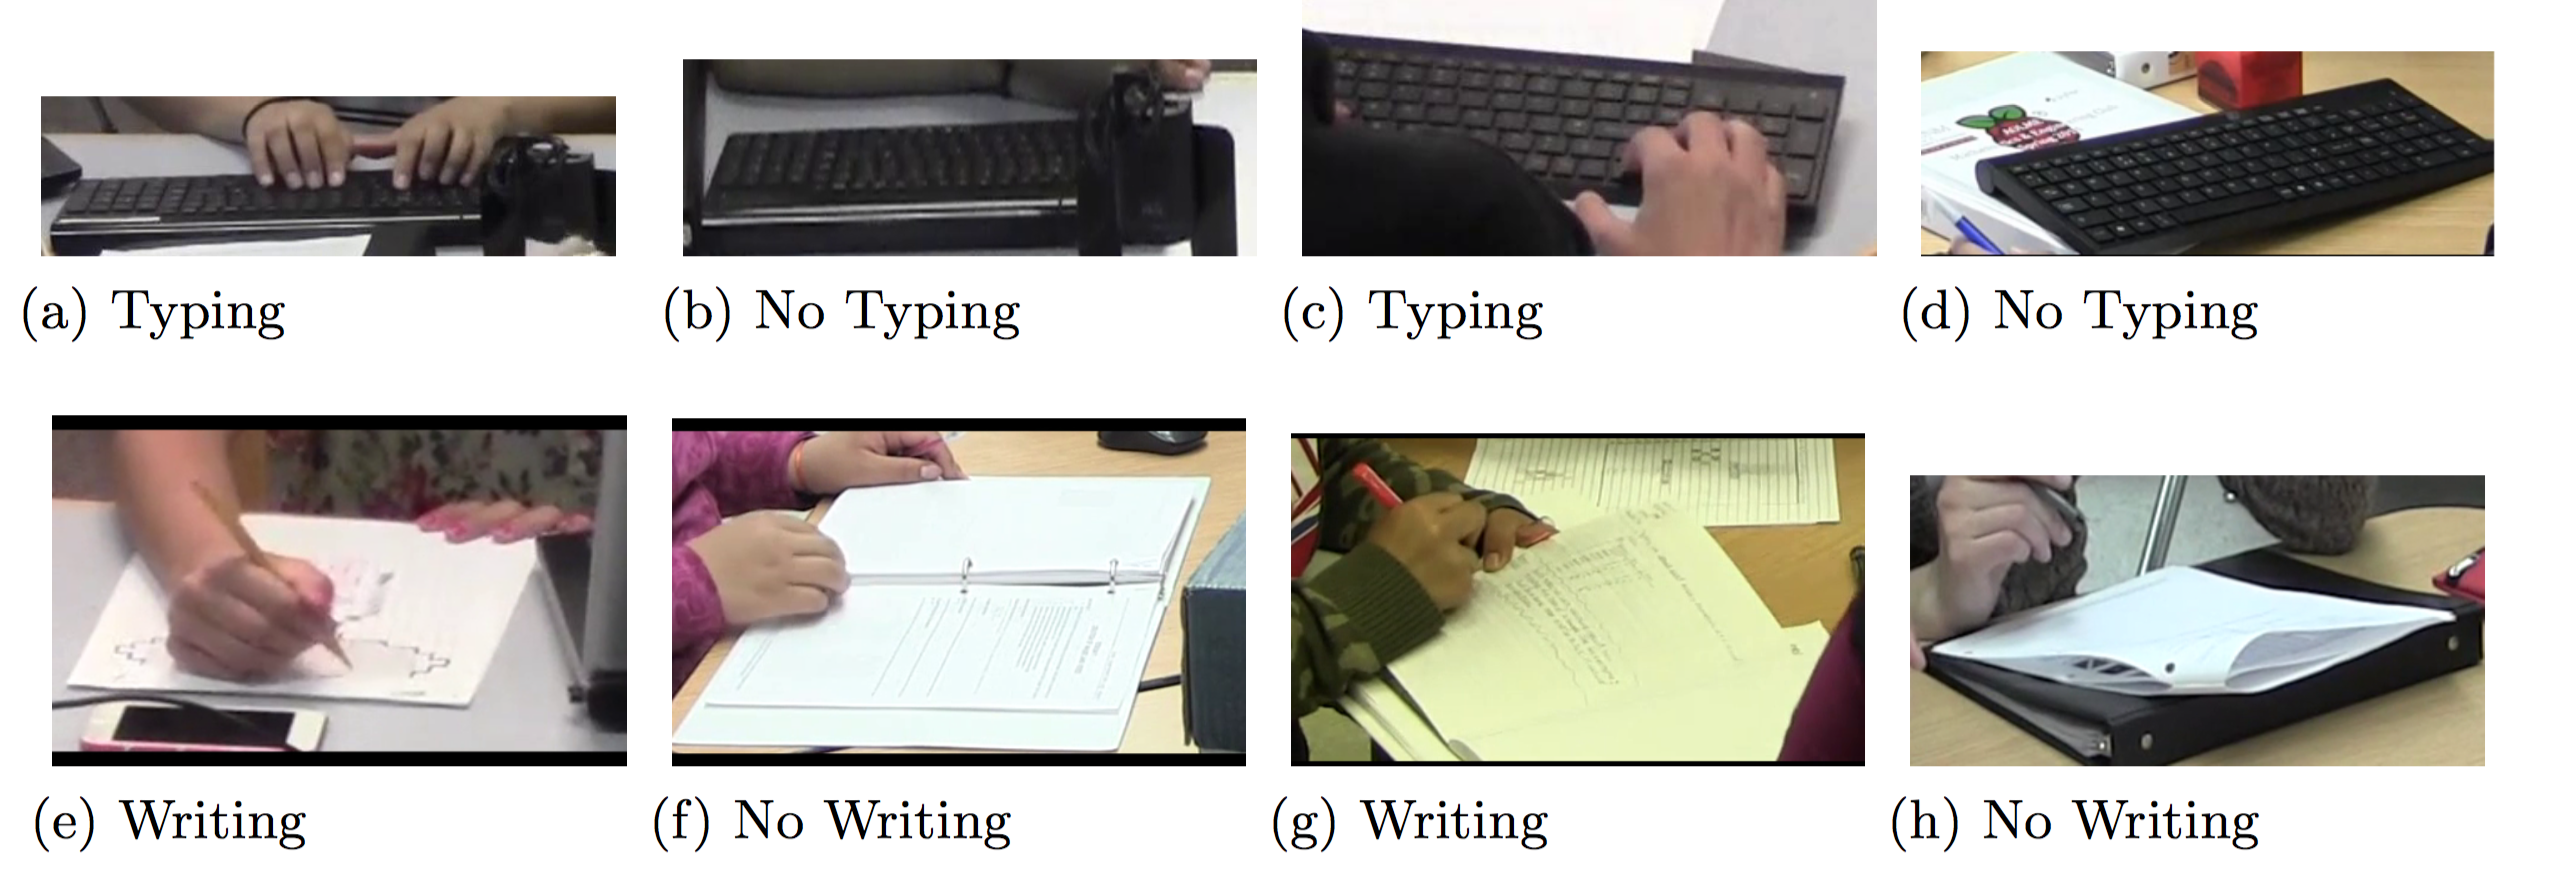
\includegraphics[width=\textwidth]{figures/typing_writing_clip}
  \caption{Example of features that have been manually extracted from the dataset
  for training and testing. For the above example, we need to classifiers for each
  activity to determine if the activity is being performed, or it is not.}
\end{figure}

\section{\label{section:contributions}Contributions}
This thesis contributes to the computer engineering community by providing both
algorithms and an architecture for efficient, scalable and rapid processing of
extremely large video datasets. The intent of this work is to also benefit
the research being done at the UNM College of Education by providing a useful
tool for automated assistance in reviewing the large video datasets provided
by AOLME.

\section{\label{section:summary}Summary}
